\documentclass{article}
	\usepackage[utf8]{inputenc}
	\usepackage{float}
	\usepackage{pdfpages}
	\usepackage[T1]{fontenc}
	\usepackage{float}
	\usepackage{booktabs}
	\usepackage{multirow}
	\usepackage{ragged2e}
	\usepackage{makecell}
	\renewcommand{\theadfont}{\small\bfseries}
	\usepackage{tabularx}
	\usepackage[autolanguage, np]{numprint}
	\newcolumntype{Z}{ >{\centering\arraybackslash}X }
	\usepackage{makecell}
	\usepackage{url}
	\usepackage{siunitx}
	\usepackage{caption}
	\usepackage[framemethod=TikZ]{mdframed}
	\usepackage{tikz, tabularx}
	\usepackage[T1]{fontenc}
	\usepackage{charter}

%%% Document Properties and Packages used 9/20
\usepackage{amsmath}        % math formulas
\usepackage{bm}             % bold math symbols
\usepackage{multicol}       % multiple columns
\usepackage[super]{nth}     % 1st, 2nd, 3rd, 4th
\usepackage{enumitem}       % ordered list (a), (b), (c)
\usepackage{graphicx}		% insert images
\graphicspath{ {./images/} }
\usepackage{geometry}
\geometry{letterpaper, margin=1in, top=0.5in} % small margins
\usepackage{biblatex}		% bibliography
\addbibresource{HW1N1.bib}
%%%%%%%%%%%%%%%%%%%%%%%%%%%%%%%%%%%%%%%%%%%%%%%%%%%%%%%%%%%%%%%%%%%%%%%%%%%%%%%
%%% Code Listing 
\usepackage{listings}
\usepackage{xcolor}

\definecolor{codegreen}{rgb}{0,0.6,0}
\definecolor{codegray}{rgb}{0.5,0.5,0.5}
\definecolor{codepurple}{rgb}{0.58,0,0.82}
\definecolor{backcolour}{rgb}{0.95,0.95,0.92}

\lstdefinestyle{mystyle}{
	backgroundcolor=\color{backcolour},   
	commentstyle=\color{codegreen},
	keywordstyle=\color{magenta},
	numberstyle=\tiny\color{codegray},
	stringstyle=\color{codepurple},
	basicstyle=\ttfamily\footnotesize,
	breakatwhitespace=false,         
	breaklines=true,                 
	captionpos=b,                    
	keepspaces=true,                 
	numbers=left,                    
	numbersep=5pt,                  
	showspaces=false,                
	showstringspaces=false,
	showtabs=false,                  
	tabsize=2
}
\lstset{style=mystyle}
%%%%%%%%%%%%%%%%%%%%%%%%%%%%%%%%%%%%%%%%%%%%%%%%%%%%%%%%%%%%%%%%%%%%%%%%%%%%%%%
\begin{document}
	
	\noindent\textbf{Justine John "JJ" A. Serdoncillo}
	\hfill \textbf{AEM 8202: Fluid Mechanics 2} \\ \hfill \textbf{April 7, 2023}
	
	\begin{center}
		\Large{\textbf{Homework 3}}    
	\end{center}
	
	\section*{Number 2}
	
	Upon using the Falkner-Skan laminar boundary layer equations, the following plots were made for different values of $\alpha$. The figure below shows the change of $f'(\eta)$ or $u/U_{\infty}$ with respect to $\eta$. The domain used is only until $\eta = 10$ and is because if the shear stress was right, the solution converges fast to 1. Other reasons are that the  equation is sensitive to the initial condition, so marching along will produce errors which can grow fast that will not reflect the expected behavior. The shear stress was found by using a binary split guess shooting method which gives the an accurate guess within 50 iterations. In order to increase the speed of the code and it's accuracy, the shooting method will stop evaluating the ordinary differential equation (ODE) if $f'$ is above a threshold over 1. After finding the necessary shear stress, the shape factor was calculated by integrating along the entire domain by the use of a left Reimann sum. This doesn't affect the accuracy that much due to the chosen $\Delta \eta = 0.001$.
		
		\begin{figure}[H]
			\centering
			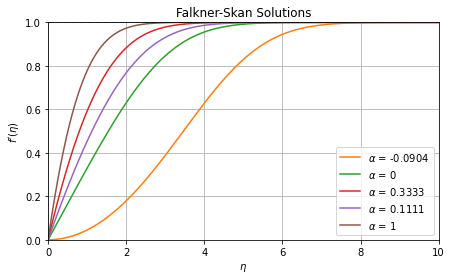
\includegraphics[width=0.6\textwidth]{images/etaOne.png}
			\caption{ Numerical solution of Falker-Skan in terms of $\eta$ }
		\end{figure}
		
		\begin{table}[h!]
			\centering
			\begin{tabular}{l l l} 
				\hline \hline
				$\alpha$ & $f''(0)$ & $H$ \\ 
				\hline
				-0.0904 & 0 & 4.0282 \\ 
				0 & 0.3321 & 2.5931 \\
				1/3 & .7574 & 2.2893 \\
				1/9 & 0.5118 & 2.409 \\
				1  & 1.2326 & 2.2334 \\
				\hline \hline
				\end{tabular}
				\caption{Vertex Coordinates of the y-direction prism}
		\end{table}
		
		In order to match the figure 10.8 in Kundu's textbook, it was noted that the $x$ scale isn't along $\eta$. Therefore it was necessary to scale it properly. It can be seen from the figure below that the produced plot looked similar to the textbook figures. 
	
		\begin{figure}[H]
			\centering
			\begin{minipage}[b]{0.48\textwidth}
				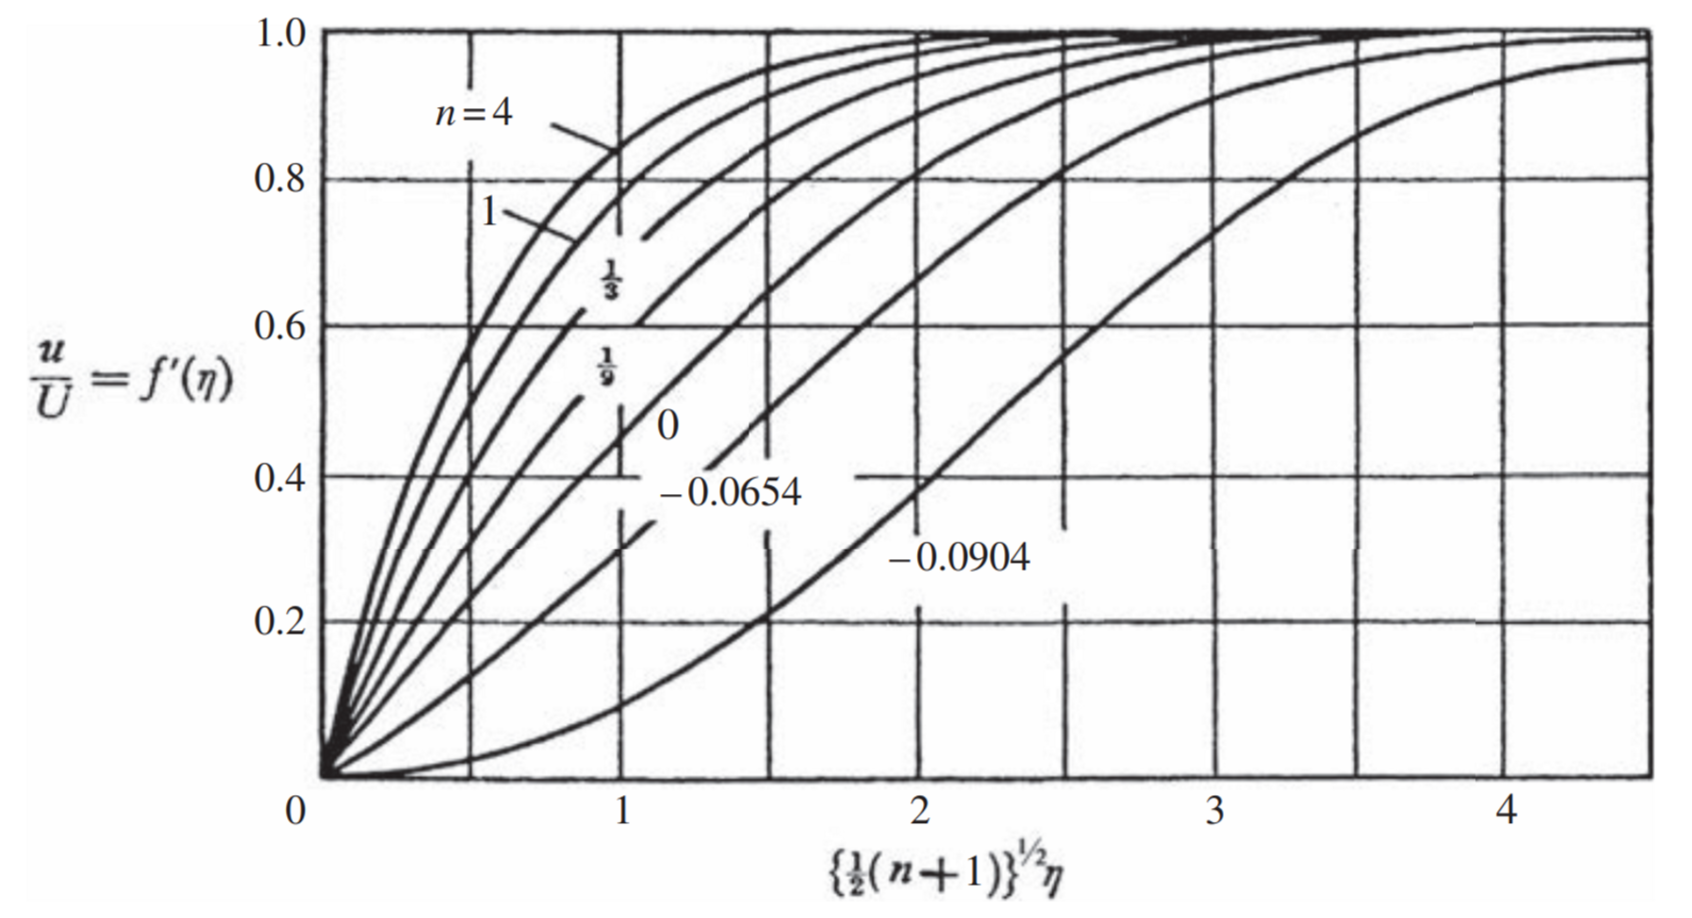
\includegraphics[width=\textwidth]{images/etaOG.png}
			\end{minipage}
			\hfill
			\begin{minipage}[b]{0.42\textwidth}
				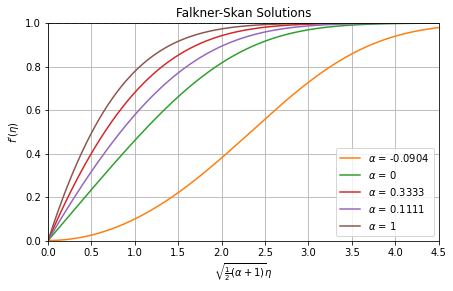
\includegraphics[width=\textwidth]{images/etaTwo.png}
			\end{minipage}
			\caption{ Comparison of Figure 10.8 from KCD and Scaled Numerical solution of Falkner-Skan  }
		\end{figure}
		
	\section*{Number 3 c)}
	
To find the velocity profile of the Non-newtonian boundary layer, a different ODE was solved. By using the same shooting method, a value of $f''(0) = 0.619$ was found. Afterwards the velocity profile was compared with the Newtonian Blasius boundary layer. It can be seen that the velocity increases faster along the $y$ axis. 
		
		\begin{figure}[H]
			\centering
			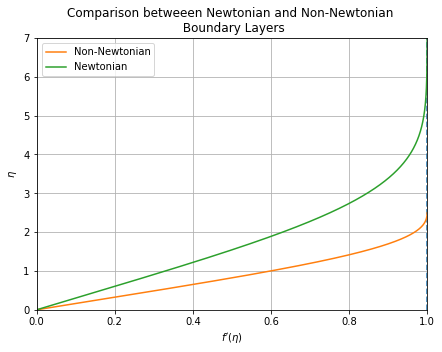
\includegraphics[width=0.6\textwidth]{images/sheesh.png}
			\caption{ Newtonian and Non-Newtonian Boundary Layers }
		\end{figure}

		
		\newpage
		\section*{Appendix)}
			\subsection*{ Python Code for Problems 2 }
			\lstinputlisting[language=Python]{HW3_P2_v5.py}
			\newpage
			\subsection*{ Python Code for Problems 3 }
			\lstinputlisting[language=Python]{HW3P3_v3.py}
	
\end{document}
